%!TEX root=finmath1.tex
\chapter{Модель \crr}
\label{ch:pr-crr}
\chaptertoc

Здесь мы реализуем модель \crr\ и вычисление в ней цен европейских и американских платежных обязательств, а также метод симуляции траекторий цены рискового актива.
В последнем разделе обсудим приближение модели \bs\ с ее помощью.

\section{Принцип реализации моделей в виде классов}
При имплементации различных моделей часто бывает удобно объединить функции, относящиеся к одной модели.
В нашем курсе для этой цели будут использоваться классы Python. 
Модель (например, модель \crr) будет представлена классом, содержащим ее параметры и набор функций для вычисления цен деривативов, симуляции цен базового актива и \td\ 
Мы будем пользоваться \emph{датаклассами}, что позволяет сократить вспомогательный технический код.
\begin{python}
### crr.py ###
from dataclasses import dataclass, field
# ... [другие импорты]

@dataclass
class CoxRossRubinstein:
    s0: float
    u: float
    d: float
    r: float = 0.0
    q: float = field(init=False)   # q не инициализируется автоматически

    def __post_init__(self):
        # Вычисление риск-нейтральной вероятности
        self.q = (self.r - self.d) / (self.u - self.d)        
\end{python}

Декоратор \verb"@dataclass" "--- это удобная конструкция, которая автоматически добавляет в создаваемый класс конструктор, инициализирующий переменные, перечисленные в классе (для этого нужно указать все переменные и их типы).
Объект класса создается операцией \verb"model = CoxRossRubinstein(s0, u, d, r)".  

Использование датакласса удобно, например, тем, что не нужно писать стандартный код конструктора следующего вида.
\begin{python}
# В датаклассе такой конструктор будет создан автоматически
class CoxRossRubinstein:
    # ...
    def __init__(self, s0, u, d, r = 0.0):
      self.s0 = s0
      self.u = u
      self.d = d
      self.r = r
\end{python}

Метод \verb"__post_init__" будет вызван автоматически после завершения работы конструктора, и его можно использовать для инициализации аттрибутов класса, которые требуют вычислений.
В нашем классе таковой является риск-нейтральная вероятность \verb"q".
Чтобы она не была включена в конструктор, мы добавили \verb"field(init=False)" в ее определение.

В \verb"__post_init__" можно добавить также, например, проверку корректности параметров модели (но в пакете \verb"finmath1" такая проверка для простоты не осуществляется).
\begin{python}
class CoxRossRubinstein:
    # ...
    def __post_init__(self):
        if (self.u <= self.d) or (self.d <= -1):
            raise ValueError('Неверные параметры u, d')
        if not (self.d < self.r < self.u):
            raise ValueError('В модели присутствует арбитраж')
        # ...
\end{python}

Датаклассы предоставляют и другие удобные методы, имплементируемые автоматически: например, метод строкового представления \verb"__str__", производящий удобно читаемый вывод при использовании \verb"print(model)". 
\begin{python}
model = CoxRossRubinstein(100, 0.1, -0.1, 0.05)
print(model)  # CoxRossRubinstein(s0=100, u=0.1, d=-0.1, r=0.05, q=0.75)
\end{python}

\begin{remark}[как расширить функционал модели]
Модель \crr, реализованная в пакете \verb"finmath1", содержит лишь базовый функционал.
Если потребуется ее расширить для использования в каких-то других приложениях, то можно либо создать класс, производный от \verb"CoxRossRubinstein" и содержащий новые функции, либо добавить глобальные функции, принимающие объект класса \verb"CoxRossRubinstein" в качестве аргумента.
То же самое относится и к другим моделям пакета. 
\begin{python}
# Производный класс от CoxRossRubinstein
class CoxRossRubinsteinExtended(CoxRossRubinstein):
    def new_function(self, arg1, arg2, ...):
    # ...

# Глобальная функции
def new_function(model, arg1, arg2, ...):
    # ...

# Использование функции из производного класса
model = CoxRossRubinsteinExtended(s0=100, u=0.1, d=0.1, r=0.05)
result = model.new_function(arg1, arg2, ...)

# Использование глобальной функции
model = CoxRossRubinstein(s0=100, u=0.1, d=0.1, r=0.05)
result = new_function(model, arg1, arg2, ...)
\end{python}
\end{remark}


\section{Вычисление цен платежных обязательств}
\subsection{Европейские обязательства, не зависящие от траектории}
Реализуем функцию вычисления цены в момент $t=0$ для европейского платежного обязательства, не зависящего от траектории цены рискового актива. Напомним, что такое платежное обязательство имеет вид $X=f(S_T)$.

Согласно результату из лекции \ref{ch:crr}, его цену можно представить в виде математического ожидания функции от случайной величины, равной количеству <<шагов вверх>> цены рискового актива и имеющей биномиальное распределение с параметрами $(T,q)$ относительно риск-нейтральной вероятности:
\[
V_0^X = \frac{1}{(1+r)^T}\E^\Q X = \frac{1}{(1+r)^T} \sum_{n=0}^T f\bigl(S_0(1+u)^n(1+d)^{T-n}\bigr) C_T^n q^n (1-q)^{T-n}.
\]

Реализуемая ниже функция цены имеет два аргумента\footnote{Помимо аргумента \verb"self".}: скалярный аргумент \verb"maturity" задает время исполнения, а аргумент \verb"payoff" должен быть универсальной функцией, которая, будучи примененной к массиву значений цены рискового актива в момент $T=$\;\verb"maturity", возвращает массив значений $f(S_T)$. 
\begin{python}
### crr.py ###
class CoxRossRubinstein:
    # ...
    def path_indep_price(self, maturity, payoff):
        N = np.arange(maturity+1)
        Q = comb(maturity, N) * self.q**N * (1-self.q)**N[::-1]
        S = self.s0 * (1+self.u)**N * (1+self.d)**N[::-1]
        return np.dot(Q, payoff(S)) / (1+self.r)**maturity
\end{python}

В этой функции массив \verb"S" содержит всевозможные значения цены рискового актива в момент $T=$\;\verb"maturity", а массив \verb"Q" "--- риск-нейтральные вероятности, что цена примет соответствущие значения.
Оба массива имеют длину \verb"maturity+1", а их $n$-ые элементы соответствуют случайному событию, когда цена идет вверх ровно $n$ раз.
Функция \verb"comb" из пакета \verb"scipy.special" вычисляет массив биномиальных коэффициентов. 
Массив \verb"payoff(S)" содержит значения выплаты $X$.
Умножая его скалярно на \verb"Q" с помощью функции \verb"np.dot", получается математическое ожидание $\E^\Q X$, которое потом дисконтируется.

Заметим, что \verb"payoff(S)" может быть и многомерным массивом, если в качестве $X$ выступает массив платежных обязательств.
Чтобы \verb"path_indep_price" в таком случае корректно работала при вычислении скалярного произведения%
\footnote{Функция \verb"np.dot(x, y)", примененная к одномерному массиву \verb"x" и многомерному массиву \verb"y", возвращает сумму произведений значений \verb"x[n]" на срезы \verb"y[n]".},
каждый срез \verb"payoff(S)[n]" должен содержать значения выплат всех платежных обязательств на случайном событии, когда цена идет вверх ровно $n$ раз. Соответственно, длина массива \verb"payoff(S)" по оси 0 должна совпадать с длиной \verb"P".
Например, если \verb"payoff(S)" "--- двумерный массив, то его $n$-я строка будет содержать значения всех выплат в случае, когда цена рискового актива идет вверх $n$ раз (платежные обязательства в таком случае образуют одномерный массив).

Используя функцию \verb"path_indep_price", добавим в наш класс методы для вычисления цен европейских опционов колл и пут.
\begin{python}
### crr.py ###
class CoxRossRubinstein:
    # ...
    def call_price(self, maturity, strike):
        payoff = lambda s: np.maximum(np.subtract.outer(s, strike), 0)
        return self.path_indep_price(maturity, payoff)
    
    def put_price(self, maturity, strike):
        payoff = lambda s: np.maximum(-np.subtract.outer(s, strike), 0)
        return self.path_indep_price(maturity, payoff)
\end{python}
Здесь считается, что аргумент \verb"maturity" является скаляром, а \verb"strike" может быть как скаляром, так и одномерным массивом\footnote{Функция будет работать и для многомерного массива \verb"strike", но трудно представить, где это может потребоваться.}.
Использование массива страйков позволяет вычислить цены сразу всех нужных опционов для заданного времени исполнения.
Это удобно и, главное, быстрее, чем вычислять цены по отдельности в дополнительном цикле.

Заметим, что для задания выплаты опциона создается лямбда-функция\footnote{Лямбда-функция "--- это безымянная функция; такие функции удобно использовать в промежуточных вычислениях.}, передаваемая в \verb"path_indep_price".
В этой функции мы пользуемся операцией внешнего вычитания, которая позволяет корректно учитывать как случай скалярного страйка, так и массива страйков.
А именно, если \verb"strike" "--- массив, то вычитание его из массива значений цены рискового актива \verb"s" дает двумерный массив, каждая строка которого состоит из всех значений выплаты опциона колл с соответствущим страйком.
Для опциона пут аналогичное поведение достигается сменой знака (написать \verb"np.subtract.outer(strike ,s)" нельзя, так как получатся несогласованные размерности).
В итоге, \verb"path_indep_price" возвращает одномерный массив с ценами всех опционов для различных страйков.

В качестве примера, вычислим цену опциона колл из примера \ref{crr:example} в лекции \ref{ch:crr}, а также массив цен трех опционов в той же модели.
\begin{python}
### crr.ipynb ###
model = CoxRossRubinstein(s0=100, u=0.1, d=-0.1, r=0.05)
print(model.call_price(2, 100))             # 10.71
print(model.call_price(2, [90, 100, 110]))  # [18.88, 10.71, 5.61]
print(model.put_price(2, [90, 100, 110]))   # [0.51, 1.42, 5.39]
\end{python}


\subsection{Европейские обязательства, зависящие от траектории}
\label{pr-crr:s:path-dep}
Рассмотрим теперь платежное обязательство вида $X = f(S_0,\dots,S_T)$, зависящее от траектории цены рискового актива. 
Для вычисления его цены воспользуемся формулой
\[
V_0^X = \frac1{(1+r)^T} \E^{\Q} X = \frac1{(1+r)^T} \sum_{\omega\in\Omega} f(S_0, S_1(\omega),\dots,S_T(\omega)) \Q(\omega).
\]
Чтобы вычислить сумму, создадим массив всех исходов \verb"Omega", массив выплат \verb"X", соответствующих этим исходам, и массив \verb"Q" их вероятностей; затем перемножим \verb"X" и \verb"Q", дисконтируем и получим искомую цену.
Приведем сначала всю функцию, а потом поясним, как она работает.
\begin{python}
### crr.py ###
class CoxRossRubinstein:
    # ...
    def path_dep_price(self, maturity, payoff):
        Omega = np.unpackbits(np.arange(2**maturity, dtype='<u8').view('u1').\
            reshape((-1, 8)), axis=1, count=maturity, bitorder='little').T
        Q  = (self.q/(1-self.q))**np.sum(Omega, axis=0) * (1-self.q)**maturity
        xi = np.where(Omega, 1+self.u, 1+self.d)
        S = self.s0*np.vstack((np.ones(2**maturity), np.cumprod(xi, axis=0)))
        X = payoff(S)
        return np.dot(Q, X) / (1+self.r)**maturity
\end{python}

Здесь каждый столбец двумерного массива \verb"Omega" содержит двоичное представление одного случайного исхода, \te\ \verb"Omega[t, n]" равно 0 или 1 в зависимости от того, идет ли цена вниз или вверх на шаге $t$ при $n$-м случайном исходе.
В частности, \verb"Omega" имеет форму $(T,\, 2^T)$, где $T=$\;\verb"maturity".

Для создания массива \verb"Omega" применяется несколько нетривиальная, но эффективная процедура, состоящая в следующем.
Сначала функция \verb"np.arange" создает массив чисел от 0 до $2^T-1$, причем ее аргумент \verb"dtype='<u8'" означает, что каждый элемент этого массива должен храниться в оперативной памяти как 8-байтное неотрицательное целое число с порядком байтов от младшего к старшему\footnote{Например, число 1 будет представлено в виде последовательности байтов $1,0,0,0,0,0,0,0$, а 258 "--- в виде $2,1,0,0,0,0,0,0$ (так называемый \emph{little-endian} порядок байтов, см.\ \url{https://en.wikipedia.org/wiki/Endianness}).}.
Затем метод \verb"view" <<разворачивает>> каждый элемент в 8 однобайтных элементов, таким образом увеличивая длину массива в 8 раз.
Потом применяется \verb"reshape", делая массив двумерным, так что каждая его строка содержит 8 однобайтных чисел (и тогда строка $n$ представляет число $n$).
К полученному массиву применяется функция \verb"np.unpackbits", которая преобразует каждый элемент массива в 8 новых элементов со значениями 0 или 1 и содержащие его биты.
Аргумент \verb"axis=1" означает, что нужно работать по строкам: битовые представления чисел в каждой строке исходного массива будут записаны в соответствующую строку нового массива, а количество строк в массиве останется прежним. 
Аргумент \verb"bitorder='little'" указывает, что биты должны идти от младшего к старшему, а \verb"count=maturity" оставляет в каждой строке нового массива только только первые \verb"maturity" элементов.
Наконец, полученный массив транспонируется, чтобы представление числа $n$ было записано в столбце $n$.

\begin{remark}
Функция \verb"np.unpackbits" работает только с массивами, элементами которых является целые однобайтные числа, и именно поэтому нам пришлось вызывать дополнительно \verb"view" и \verb"reshape", вместо того, чтобы написать что-то вроде \verb"np.unpackbits(np.arange(2**maturity), count=maturity)".
\end{remark}

Далее для вычисления массива вероятностей $Q$ используется формула
\[
\Q(\omega) = \left(\frac{1+u}{1+d}\right)^{\sum_{n=1}^T a_n} (1+d)^T,
\]
где каждый исход $\omega=(a_1,\dots,a_T)$ соответствует одному столбцу массива \verb"Omega", и поэтому при вычислении суммы мы указываем аргумент \verb"axis=0", суммирующий по строкам.

Массив \verb"xi" получается из \verb"Omega" заменой 0 на $1+d$, а 1 на $1+u$, для чего используется функция \verb"np.where".
В общем случае \verb"np.where(x, a, b)" принимает массив логических значений \verb"x" и возвращает массив такой же формы, где на месте каждого истинного значения записано \verb"a", а на месте ложного "--- \verb"b" (при этом \verb"a" и \verb"b" могут быть массивами, тогда из них будут выбираться элементы с соответствующими индексами; подробнее см.~документацию\footnote{\url{https://numpy.org/doc/2.2/reference/generated/numpy.where.html}}).
В нашем случае нулевые элементы \verb"Omega" трактуются как ложные, а единичные как истинные. 

Двумерный массив \verb"S" в каждом своем столбце содержит траекторию цены рискового актива (и, следовательно, имеет форму $(T+1,\, 2^T)$).
Для его создания используется формула
\[
S_0 = s_0, \qquad S_t = S_{t-1}\xi_t,\ t=1,\dots,T,
\]
вычисление которой выполняется применением функции кумулятивного произведения вдоль столбцов массива \verb"xi", добавлением сверху строки из единиц и умножением на начальное условие. 

Массив выплат \verb"X" получается применением передаваемой функции \verb"payoff" к \verb"S". Считается, что она возвращает одномерный массив, состоящий из значений выплаты платежного обязательства на каждой траектории%
\footnote{Все будет работать и в случае нескольких платежных обязательств.
Тогда \verb"payoff" должна возвращать многомерный массив, у которого каждый срез \verb"payoff(S)[n]" представляет значения выплат всех платежных обязательств на траектории $S(\omega_n)$.}.

Наконец, массив вероятностей умножается на массив выплат, что дает математическое ожидание $\E^{\Q} X$, которое потом дисконтируется.

Проверим работу реализованного алгоритма сначала на каком-нибудь простом случае.
В качестве примера, вычислим с его помощью цену опциона колл из предыдущего раздела.
\begin{python}
model = CoxRossRubinstein(s0=100, u=0.1, d=-0.1, r=0.05)
print(model.path_dep_price(2, lambda s: np.maximum(s[-1] - 100, 0)))  # 10.71
\end{python}
Здесь функция выплаты устроена так, что из массива траекторий цены рискового актива она берет только последнюю строку (значения $S_T$) и вычисляет выплату опциона колл со страйком 100.
Получается тот же результат, что и при использовании \verb"path_indep_price" и \verb"call_price".

Теперь приведем более содержательный пример и вычислим цену барьерного опциона вниз-и-выход из примера \ref{crr:e:barrier} в лекции \ref{ch:crr}.
\begin{python}
### crr.ipynb ##
T = 2
K = 95
H = 92
barrier_payoff = lambda s: np.maximum(s[-1] - K, 0) * np.all(s>=H, axis=0)
print(model.path_dep_price(T, barrier_payoff))  # 13.95
\end{python}
Здесь выплата опциона колл умножается на индикатор того, что цена находилась не ниже барьера $H$.
Заметим, что выражение \verb"s>=H" является массивом (такой же формы как \verb"s") и содержит значения \verb"True" или \verb"False" в зависимости от того, находится ли каждое значение цены не ниже барьера.
Функция \verb"np.all" реализует операцию логического <<и>>.
В данном случае она применяется по строкам (\verb"axis=0"), \te\ получается одномерный массив, каждый элемент которого будет равен \verb"True", если все элементы соответствующего столбца массива \verb"s>=H" истинны, и \verb"False" иначе.
При умножении числового массива \verb"np.maximum(s[-1] - K, 0)" на получившийся логический массив значение \verb"True" трактуется как 1, а \verb"False" как 0, что и соответствует умножению на индикатор.

\begin{remark}
Представление выплат сложных деривативов в виде универсальной функции может быть иногда затруднительно.
Вместо этого можно написать функцию выплаты, применяемую к одной траектории, а в \verb"path_dep_price" передать лямбда-функцию, которая будет применять ее к каждому столбу передаваемого двумерного массива цен (хотя это приведет к потере скорости).

Например, предыдущий фрагмент можно было бы переписать следующим образом.
\begin{python}
barrier_payoff = lambda s: max(s[-1] - K, 0) * np.all(s>=H)
print(model.path_dep_price(T, lambda S : [barrier_payoff(s) for s in S.T]))
\end{python}
Здесь считается, что в \verb"barrier_payoff" передается одномерный массив \verb"s", а поэтому \verb"s[-1] - K" является скаляром, и можно воспользоваться встроенной функцией \verb"max" вместо \verb"np.maximum".
Кроме того, не нужно указывать \verb"axis=0" при вызове \verb"np.all". 
Далее при вызове \verb"path_dep_price" создается лямбда-функция, которая применяет функцию выплаты к каждому столбцу передаваемого двумерного массива \verb"S" (конструкция \verb"s in ..." проходит по строкам массива, а так как нам нужны столбцы, то нужно транспонировать \verb"S").
\end{remark}


\subsection{Американские обязательства}
Для вычисления цен американских платежных обязательств воспользуемся методом обратной индукции.
Мы будем рассматривать платежные обязательства, выплата которых при исполнении в момент времени $t$ зависит только от цены базового акива в этот момент, т.е.\ $X_t=f(S_t)$, где $f(s)$ "--- детерминированная функция.
Такой вид, в частности, имеют функции выплат американских опционов колл и пут.
\begin{python}
### crr.py ###
class CoxRossRubinstein:
    # ...
    def american_price(self, maturity, payoff):
        def X(t):
            N = np.arange(t+1)
            return payoff(self.s0 * (1+self.u)**N * (1+self.d)**(t-N))
        V = X(maturity)
        for t in range(maturity-1, -1, -1): # t пробегает от maturity-1 до 0
            V[:t+1] = np.maximum(X(t),
                (self.q*V[1:t+2] + (1-self.q)*V[:t+1])/(1+self.r))
        return V[0]    
\end{python}
Сначала здесь создается вспомогательная функция \verb"X", вычисляющая массив всех возможных значений выплаты $X_t$.
Предполагается, что \verb"payoff", играющая роль указанной выше функции $f$, является универсальной функцией, которая применяется к массиву значений цены базового актива и возвращает соответствующий массив значений выплат платежного обязательства. 

Далее реализуется собственно алгоритм обратной индукции.
Мы пользуемся тем, что, в силу марковского свойства цены базового актива, справедливо равенство $V_{t} = V(t, S_{t})$, где функция $V(t,s)$ имеет вид
\begin{align*}
&V(T, s) = f(s), \\
&V(t, s) = \max(f(s),\ (1+r)^{-1}\E^\Q(V({t+1}, S_{t+1}) \mid S_t=s))\ \text{при}\ t < T,
\end{align*}
причем присутствующее здесь условное математическое ожидание можно вычислить по формуле
\[
\E^\Q(V({t+1}, S_{t+1}) \mid S_t=s) = qV(t+1, s(1+u)) + (1-q)V(t+1, s(1+d)).
\]
По ходу обратной индукции значения функции $V(t,s)$ на шаге $t=T,T-1,\dots,0$ записываются в массив \verb"V", перезаписывая его первые $t+1$ элементов, так что элемент \verb"V[n]", где $n=0,\dots,t$, представляет значение функции $V(t, s)$ для $s=s_0(1+u)^n(1+d)^{t-n}$.
Искомое значение цены в начальный момент времени будет записано в \verb"V[0]" на последнем шаге цикла.

Используя написанную общую функцию, добавим в класс также методы вычисления цен американских опционов колл и пут (в этих функциях предполагается, что оба аргумента \verb"maturity" и \verb"strike" являются скалярами).
\begin{python}
### crr.py ###
class CoxRossRubinstein:
    # ...
    def american_call_price(self, maturity, strike):
        return self.american_price(lambda s: np.maximum(s-strike, 0), maturity)

    def american_put_price(self, maturity, strike):
        return self.american_price(lambda s: np.maximum(strike-s, 0), maturity)
\end{python}

В качестве иллюстрации, найдем цену американских опционов колл и пут со страйком $K=102$ для двухшаговой модели приведенной выше (цену пут мы нашли в примере \ref{am-d:e:price} в лекции \ref{ch:american-discrete}).
Заметим, что цена американского опциона колл совпадает с ценой европейского опциона колл, как и должно быть при неотрицательной процентной ставке в отсутствие дивидендов, см.~раздел \ref{am-d:s:equal-prices} в лекции \ref{ch:american-discrete}.
Цены опционов пут различаются.
\begin{python}
### crr.ipynb ###
print(model.american_call_price(2, 102))  # 9.69 (американский колл)
print(model.call_price(2, 102))           # 9.69 (европейский колл)
print(model.american_put_price(2, 102))   # 3.37 (американский пут)
print(model.put_price(2, 102))            # 2.21 (европейский пут)
\end{python}


\section{Симуляция цены рискового актива}
Реализуем функцию, симулирующую траектории цены рискового актива, чтобы использовать их, например, в методе \mc.
Так как гораздо эффективнее симулировать траектории не по одной, а группами (чтобы использовать векторизацию), то нам нужна функция, возвращающая двумерный массив из заданного количества траекторий.
Везде далее будет предполагаться, что одна траектория представлена столбцом этого массива, и, таким образом, массив должен иметь форму $(T+1, M)$, где $M$ "--- требуемое количество траекторий.
Мы включаем в каждую траекторию начальное значение $S_0$, поэтому число строк в массиве равно $T+1$.

Траектории всегда будут симулироваться относительно риск-нейтральной вероятности. 
Воспользуемся тем, что относительно нее справедливо представление
\[
S_t = S_{t-1}\xi_t,
\]
где $\xi_1,\dots,\xi_T$ "--- независимые случайные величины, принимающие значения $1+u$ и $1+d$ с вероятностями $q$ и $1-q$.

\begin{python}
### crr.py ###
class CoxRossRubinstein:
    # ...
    def simulate(self, t, paths, rng=None):
        if rng is None:
            rng = np.random.default_rng()  
        xi = np.where(rng.uniform(size=(t, paths)) < self.q, 1+self.u, 1+self.d)
        return self.s0*np.vstack((np.ones(paths), np.cumprod(xi, axis=0)))
\end{python}
Эта функция принимает целочисленные аргументы \verb"t" (последний момент времени) и \verb"paths" (количество траекторий), а также объект генератора случайных чисел 
\verb"rng". Если \verb"rng" равен \py{None}, то будет использован генератор по умолчанию.
Если нужна воспроизводимость результатов, то следует передать заранее созданный генератор с фиксированным начальным состоянием (см.~замечание \ref{np:r:seed} в практикуме \ref{ch:numpy}).

Массив \verb"xi" составлен из столбцов, содержащих значения $\xi_1,\dots,\xi_T$ для каждой симулированной траектории: \verb"rng.uniform(size=(t, paths)) < self.q" дает двумерный массив, составленный из значений \verb"True" или \verb"False" с вероятностями $q$ и $1-q$, а затем к нему применяется функция выбора \verb"np.where" подобно тому, как это делалось разделе \ref{pr-crr:s:path-dep}.
Из массива \verb"xi" получается массив траекторий цен, опять же, аналогично коду в разделе \ref{pr-crr:s:path-dep}.

В качестве примера, приводимый ниже фрагмент кода симулирует небольшое число траекторий и строит их графики.
В следующем практикуме мы увидим, как пользоваться этой функцией в методе \mc.
\begin{python}
### crr.ipynb ###
# 5 траекторий в 50-шаговой модели
model = CoxRossRubinstein(s0=100, u=0.02, d=-0.02)
plt.plot(model.simulate(50, 5))
plt.xticks(range(0, 51, 10));  # Сделать отметки по оси x через каждые 10 шагов
\end{python}

\noindent
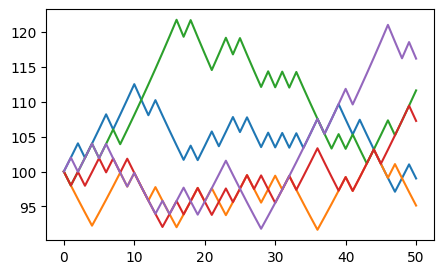
\includegraphics[width=7cm]{pic/crr-path-many.png}


\section{Приближение модели \bs}
Как показано в дополнительном материале \ref{ch:crr-limit}, модель \crr\ сходится к модели \bs\ при числе шагов $T\to\infty$ и параметрах $u,d,r\to0$, и, в частности, сходятся цены платежных обязательств (при некоторых условиях на интегрируемость функции выплат).
Продемонстрируем это на примере сходимости цен европейских опционов колл.

Рассмотрим модель \bs\ с фиксированными параметрами $s_0$, $\sigma$, $r$ и модель \crr\ такой же начальной ценой $s_0$ и параметрами
\[
u = \frac{\sigma}{\sqrt n}, \qquad d = -\frac{\sigma}{\sqrt n}, \qquad r' = \frac{r}{n}.
\]
Построим графики цен опционов колл с моментом исполнения $T$ в модели \bs\ и моментом исполнения $Tn$ в модели \crr, где $T$ "--- <<календарное>> время (чтобы избежать дополнительных трудностей с округлением, будем считать, что $T$ "--- целое), а также построим графики их подразумеваемой волатильности (см.~замечание ниже о том, зачем это делать).
Следующий фрагмент кода иллюстрирует это для $n=10$ и $n=100$.
В нем используется класс \verb"BlackScholes", а также функция вычисления подразумеваемой волатильности \verb"implied_vol", которые будут разбираться в дальнейших практикумах.
\begin{python}
### crr.ipynb ###
s0 = 100
sigma = 0.3
r = 0.05
T = 1

# Создадим 4 подграфика и отрегулируем горизонтальный промежуток между ними
fig, ax = plt.subplots(2, 2, figsize=(10,6), squeeze=False)
fig.subplots_adjust(hspace=0.4)

# Модель Блэка-Шоулса и цены опционов в ней
bs_model = BlackScholes(s0, sigma, r)     
K = np.linspace(50, 200, 100)   # диапазон страйков
bs_price = bs_model.call_price(T, K)

for i, n in enumerate([10, 100]):
    # Цены опционов и их волатильность в модели Кокса-Росса-Рубинштейна
    crr_model = CoxRossRubinstein(s0, sigma/sqrt(n), -sigma/sqrt(n), r/n)
    crr_price = crr_model.call_price(T*n, K)
    crr_iv = implied_vol(s0*exp(r*T), T, K, crr_price, discount_factor=exp(-r*T))

    # Слева будут графики цен
    ax[i,0].plot(K, bs_price, label="Блэк-Шоулс")
    ax[i,0].plot(K, crr_price, label="Кокс-Росс-Рубинштейн")
    ax[i,0].legend(loc="upper right", frameon=False)
    ax[i,0].set_title(f"Цены опционов (n={n})", fontsize=10, fontweight="bold")
    ax[i,0].set_xlabel("Страйк")
    ax[i,0].set_ylabel("Цена")

    # а справа - графики волатильности
    ax[i,1].plot(K, np.ones(len(K))*sigma, label="Блэк-Шоулс")
    ax[i,1].plot(K, crr_iv, label="Кокс-Росс-Рубинштейн")
    ax[i,1].set_ylim(0.25, 0.35)
    ax[i,1].legend(loc="upper right", frameon=False)
    ax[i,1].set_title(f"Подразумеваемая волатильность (n={n})", fontsize=10,
        fontweight="bold")
    ax[i,1].set_xlabel("Страйк")
    ax[i,1].set_ylabel("Волатильность")
\end{python}

\noindent
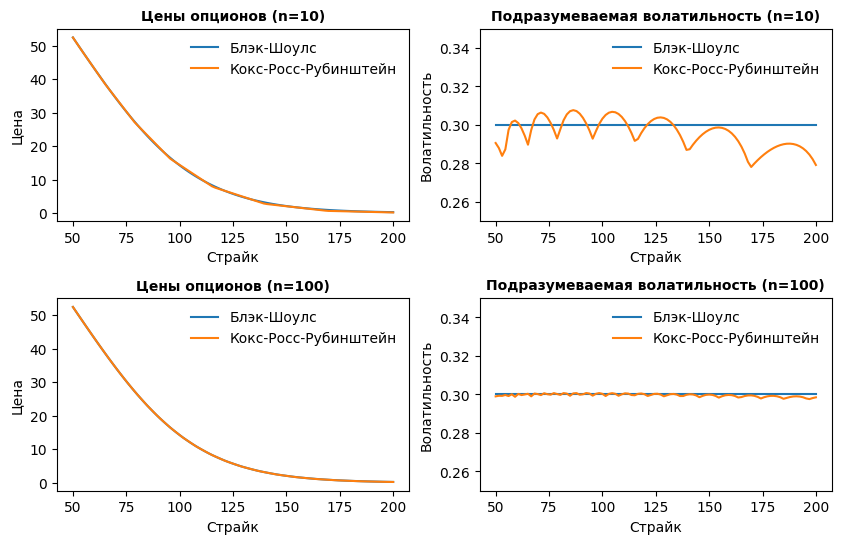
\includegraphics[width=14cm]{pic/crr-limit.png}

\begin{remark}
Мы приводим графики подразумеваемой волатильности потому, что она позволяет лучше понять, насколько качественным является построенное приближение.
На графиках видно, что цены опционов для модели \crr\ и \bs\ близки и при $n=10$, и при $n=100$, но при $n=10$ приближение волатильности получается недостаточно хорошим (ошибка около 2\%, которая здесь получается, на практике не считается пренебрежительной).
\end{remark}
